\documentclass{beamer}

\usepackage{epsfig}
\usepackage{multicol}
\usepackage{geometry}
%\usepackage[dvipsnames]{xcolor}
\usepackage{textcomp}
\usepackage{graphicx}
\usepackage{caption}
\usepackage{subcaption}
\usepackage{amsmath}
\usepackage{tcolorbox}
\usetheme{Boadilla}
\usepackage{pict2e}
\usepackage{tikz}
\usepackage{xcolor}

\title[Modelling Dec 2023]{Presentation : Modelling studies Dec 2023}
\author[Antony Bazir]{}


\setlength{\unitlength}{1cm}

\begin{document}
\begin{frame}
\centering 
\textbf{Presentation : \\ Modelling Studies \\  Dec 2023}\\
\vspace{0.5 cm}
Antony BAZIR
\end{frame}

\section{Context}
\begin{frame}
\frametitle{Context : Standalone Modelling Study}
\begin{columns} 
		\column{50mm}
			\vspace{0cm}\\
				\includegraphics[width=45mm]{/home/antonybazir/Documents/Post-doc/test_fortran/plots/0823/cells_A120g.pdf}\\
				\vspace{0.1cm}
				\includegraphics[width=45mm]{/home/antonybazir/Documents/Post-doc/test_fortran/plots/0823/G_A120g.pdf}\\
			\textit{\tiny Cell population and nutrient distribution in the chip model}
			 
		
		\column{50mm}
		\underline{Last time :}
			\begin{itemize}
				\item Cell divisions and nutrient dynamics in the chip
				\item Range of parameters found in the literature and tested
			\end{itemize}
			However, full experiments not yet available for comparison
			
				\begin{block}{}
					Goal : find a useful related study to focus in the meantime
				\end{block}
			
	\end{columns} 
	
\end{frame}

\begin{frame}
	\frametitle{Context : Standalone Modelling Study}
	
	\textbf{First approach : Quantitative Metabolism of a single cell line
	}
	
	\vspace{2cm}
	
	\begin{enumerate}
		\item Gather data from several studies on glucose and oxygen consumption
		\item Use data to formulate consumption and growth functions for different conditions 
		\item Use the model to interpolate/extrapolate on the available data  
	\end{enumerate}
	
	\vspace{1cm} 
	
	\only<2>{On paper, this looks good...}
\end{frame}

\begin{frame}
	\frametitle{Context : Standalone Modelling Study}
	
	\textbf{First approach : Quantitative Metabolism of a single cell line \textbf{MCF-7}
	}
	
	\vspace{1cm}
	\underline{Problems :}
	\begin{enumerate}
		\item Quantitative consumption data comes in all shapes and sizes...
		\item Data needed for conversion might be lacking or incomplete
		\item Even after attempting to account for all this, still significant spread in the data... 
	\end{enumerate}
	
	\only<2>{\begin{block}{}
		Let us try something else...
	\end{block}}

\end{frame}

\begin{frame}
	\frametitle{Context : Standalone Modelling Study}
	
	\textbf{Second approach : General growth and metabolism of cancer cell lines in various configuration
	}
	
	\vspace{1cm}
	\begin{enumerate}
		\item Study the literature and try to find metabolic behaviors common to all cell lines (ex : Glycolytic switch)
		\item Model different culture configurations (2D, 3D w or w/o scaffold etc...)  
	\end{enumerate}
	
	\only<2>{\begin{block}{}
		HOWEVER
	\end{block}}

\end{frame}


\begin{frame}
	\frametitle{Context : Standalone Modelling Study}
	
	\textbf{Second approach : General growth and metabolism of cancer cell lines in various configuration
	}
	
	\vspace{1cm}
	\underline{Problems :}
	\begin{enumerate}
		\item Closer literature review suggest that uncontrolled proliferation and glycolytic switch are the only widespread characteristics
		\item Some lines can use glutamine, or lactate, or reverse the TCA cycle, etc...
		\item Attempts to formulate a problematic resulted in things that were too simple (or already done) or too complex...  
	\end{enumerate}
	
	\only<2>{\begin{block}{}
		Foiled again...
	\end{block}}

\end{frame}

\begin{frame}
	\frametitle{Context : Standalone Modelling Study}
	
	\textbf{Third approach : General growth and metabolism model focused on qualitative differences
	}
	
	\vspace{1cm}

	\begin{enumerate}
		\item Sort out and pick essential components of the link between metabolism and growth
		\item Simplify and group the different metabolic responses observed in cells 
		\item Build a modelling tool growth trend and nutrient dynamics to metabolic response at the cellular level  
	\end{enumerate}
	
	\only<2>{\begin{block}{}
		And so work started...
	\end{block}}

\end{frame}

\begin{frame}
\frametitle{Metabolic Variety : Basic Ideas}

	 \begin{columns}
	 	\column{50mm}
		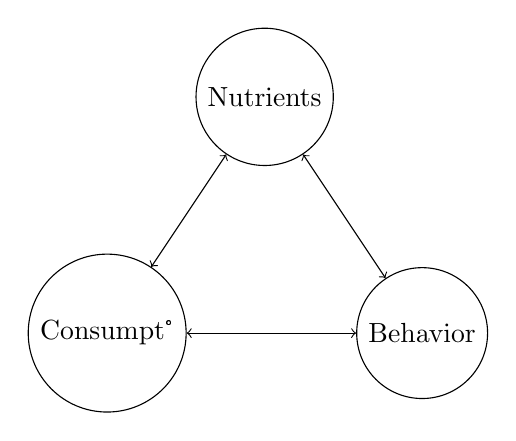
\begin{tikzpicture}
		\node[circle,draw] (B) at (2,0) {Behavior};
		\node[circle,draw] (C) at (-2,0) {Consumpt°};
		\node[circle,draw] (N) at (0,3) {Nutrients};
		
		\draw[<->] (B)--(C);
		\draw[<->] (C)--(N); 
		\draw[<->] (N)--(B); 
		\end{tikzpicture}
		
		\column{40mm}
		\begin{itemize}
		\item  Hybrid agent-based model
		\item  Gradual complexification of the behavior of cells/agents
		\item Search for the different trends in growth and nutrients dynamics 
		\end{itemize}
	\end{columns}
\end{frame}


\section{Model structure}
\begin{frame} 
\frametitle{Metabolic Variety : Model structure}
Keeping it simple:  Cells and nutrients modelled on 2D square grids\\
\vspace{0.5cm}
\begin{columns}[T]
\column{30mm}
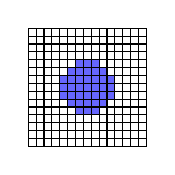
\begin{tikzpicture}
	\draw (0,0) grid[step=0.1] (1.5,1.5) rectangle (0,0);
	
    \draw[fill=blue!60!white] (0.5,0.5) grid[step=0.1] (1.0,1.0) rectangle (0.5,0.5);
    \draw[fill=blue!60!white] (0.4,0.6) grid[step=0.1] (1.1,0.9) rectangle (0.4,0.6);
 	\draw[fill=blue!60!white] (0.6,0.4) grid[step=0.1] (0.9,1.1) rectangle (0.6,0.4);
 	%\draw[->]
\end{tikzpicture}\\
\vspace{0.5cm}
\small{
Cell grid :}\scriptsize{
\begin{itemize}
\item Keeps track of individual cells
\item Linked to a global state vector 
\end{itemize}
}
 \column{30mm}
 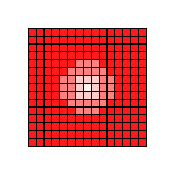
\begin{tikzpicture}	
 	\draw[fill=red!90!white] (0,0) grid[step=0.1] (1.5,1.5) rectangle (0,0);
	
    \draw[fill=red!50!white] (0.5,0.5) grid[step=0.1] (1.0,1.0) rectangle (0.5,0.5);
    \draw[fill=red!50!white] (0.4,0.6) grid[step=0.1] (1.1,0.9) rectangle (0.4,0.6);
 	\draw[fill=red!50!white] (0.6,0.4) grid[step=0.1] (0.9,1.1) rectangle (0.6,0.4);
 		\draw[fill=red!20!white] (0.6,0.6) grid[step=0.1] (0.9,0.9) rectangle (0.6,0.6);
 		\draw[fill=red!5!white] (0.7,0.7) grid[step=0.1] (0.8,0.8) rectangle (0.7,0.7);
\end{tikzpicture}\\
\vspace{0.5cm}
\small{
Nutrients grid :}\\
\scriptsize{
\begin{itemize}
\item Modelled w/ reaction diffusion equation
\item Solved w/ finite differences
\item ext. conc. kept constant
\end{itemize}
}
 \column{30mm}
 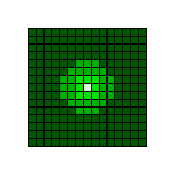
\begin{tikzpicture}	
 	\draw[fill=green!35!black] (0,0) grid[step=0.1] (1.5,1.5) rectangle (0,0);
	
    \draw[fill=green!70!black] (0.5,0.5) grid[step=0.1] (1.0,1.0) rectangle (0.5,0.5);
    \draw[fill=green!70!black] (0.4,0.6) grid[step=0.1] (1.1,0.9) rectangle (0.4,0.6);
 	\draw[fill=green!70!black] (0.6,0.4) grid[step=0.1] (0.9,1.1) rectangle (0.6,0.4);
 		\draw[fill=green!90!black] (0.6,0.6) grid[step=0.1] (0.9,0.9) rectangle (0.6,0.6);
 		\draw[fill=green!15!white] (0.7,0.7) grid[step=0.1] (0.8,0.8) rectangle (0.7,0.7);
\end{tikzpicture}\\
\vspace{0.5cm}
\small{
Consumption grid :}\scriptsize{
\begin{itemize}
\item keeps track of metabolic states
\item also used for solving RD eq.
\end{itemize}
}
\end{columns}
\end{frame}

\subsection{Population Growth}

\subsection{Nutrients Dynamics}
\begin{frame}
\frametitle{Metabolic Variety : Nutrients dynamics}
Solving non-dimensionalised reaction-diffusion equation\\
\begin{center}
\vspace{1 cm}
$ \tau \frac{d C}{\partial t}  = d_0^2 \nabla \frac{D}{D_{ox,med}} \nabla C + d_0^2 \frac{D}{D_{ox,med}} \Delta C + \frac{\tau k_C}{C_{ext}} \frac{C}{\frac{Cm}{C_{ext}} + C}  $\\
\vspace{0.4cm}
\end{center}
\scriptsize{\hspace{3.5cm} \only<2->{diffusion terms}  \hspace{1.7 cm} \only<3->{consumption term}}

\vspace{0.7 cm}
\only<4->{
\small{
\begin{itemize}
\item $C$ is normalised by external concentration (1 outside tissue)
\item $D_{ox,med}$ : Diff. coeff. of O$_2$ in surr. medium 
\item $d_0$: cell diam. / $\tau = \frac{d_0^2}{D_{ox,med}}$
\end{itemize} 
}
}
\end{frame}

\begin{frame}
\frametitle{Metabolic Variety : Nutrients dynamics}
Determination of spatial and temporal parameters for resolution:\\
\vspace{0.3 cm}
\begin{tikzpicture}
\draw[->] (0,0)--(11,0);
\foreach \x in {0,1,...,10} \draw(\x,-0.1)--(\x,0.1);
\draw (11,-0.3) node {$t_{max}$};
\draw (1,-0.3) node {$\Delta t$};
\draw (0,-0.3) node {$0$};

\begin{scope}[yshift=-1.5cm]
\draw[-] (0,0)--(11,0);
\foreach \x in {0,1,...,11} \draw(\x,-0.1)--(\x,0.1);
\draw (11,-0.3) node {$x_{max}$};
\draw (0,-0.3) node {$x_{min}$};
\draw (1,-0.3) node {$\Delta x$};
\end{scope}
\end{tikzpicture}

\small{
\begin{itemize} 
\item<2->  $t_{max} \approx 1000$ mn \hspace{1cm} $x_{max} \approx 1$ mm
\item<3->  Num. stability $\rightarrow \frac{\Delta x^2}{2 \Delta t} > D_{O_2,med}$
\item<4-> $\Delta x \approx$ cell diam. $\rightarrow$ $\Delta x \approx$ 10 - 100 \textmu m $\rightarrow$ $\Delta t \approx $ 0.0005 - 0.05 mn
\item<5-> 1000 sim mns $\rightarrow$ 30 real mns \tiny{($\Delta x = 20$ \textmu m, 100x100 grid}) \small{or 4 real mns }\tiny{($\Delta x = 60$ \textmu m 100x100 grid )}
\end{itemize} 
}
	\only<6>{\begin{block}{}
		In practice, several cycles for each configuration and several configurations ($\approx$ 20) $\rightarrow  \Delta x = 60$ \textmu m
	\end{block}}
\end{frame}


\begin{frame}
\frametitle{Metabolic Variety : Population growth}
How do cells divide in the circular patch ?\\
\vspace{0.5 cm}
\begin{columns}[T]

\column{30mm}
\only<2->{
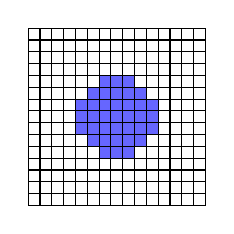
\begin{tikzpicture}
\begin{scope}[scale=1.5]
	\draw (0,0) grid[step=0.1] (1.5,1.5) rectangle (0,0);
	
    \draw[fill=blue!60!white] (0.5,0.5) grid[step=0.1] (1.0,1.0) rectangle (0.5,0.5);
    \draw[fill=blue!60!white] (0.4,0.6) grid[step=0.1] (1.1,0.9) rectangle (0.4,0.6);
 	\draw[fill=blue!60!white] (0.6,0.4) grid[step=0.1] (0.9,1.1) rectangle (0.6,0.4);
\end{scope}	
\end{tikzpicture}\\
\vspace{0.3 cm}
\scriptsize{
Cell can divide at the rim or in the patch 
}
}


\column{30mm}
\only<3->{
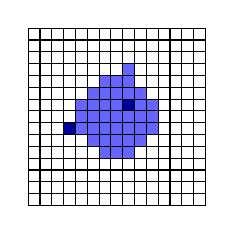
\begin{tikzpicture}
\begin{scope}[scale=1.5]
	\draw (0,0) grid[step=0.1] (1.5,1.5) rectangle (0,0);
	
    \draw[fill=blue!60!white] (0.5,0.5) grid[step=0.1] (1.0,1.0) rectangle (0.5,0.5);
    \draw[fill=blue!60!white] (0.4,0.6) grid[step=0.1] (1.1,0.9) rectangle (0.4,0.6);
 	\draw[fill=blue!60!white] (0.6,0.4) grid[step=0.1] (0.9,1.1) rectangle (0.6,0.4);
 	
 	 	\draw[fill=blue!60!black] (0.3,0.6) grid[step=0.1] (0.4,0.7) rectangle (0.3,0.6);
 	 	\draw[fill=blue!60!white] (0.8,1.1) grid[step=0.1] (0.9,1.2) rectangle (0.8,1.1);
 	 	\draw[fill=blue!60!black] (0.8,0.8) grid[step=0.1] (0.9,0.9) rectangle (0.8,0.8);
%draw[->] (1,0.5)--(1.5,0.5);
\end{scope}	

\end{tikzpicture}\\
\vspace{0.3 cm}
\scriptsize{
division in the patch shifts neighbors 
}
}


\column{30mm}
\only<4->{
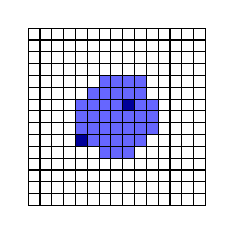
\begin{tikzpicture}
\begin{scope}[scale=1.5]
	\draw (0,0) grid[step=0.1] (1.5,1.5) rectangle (0,0);
	
    \draw[fill=blue!60!white] (0.5,0.5) grid[step=0.1] (1.0,1.0) rectangle (0.5,0.5);
    \draw[fill=blue!60!white] (0.4,0.6) grid[step=0.1] (1.1,0.9) rectangle (0.4,0.6);
 	\draw[fill=blue!60!white] (0.6,0.4) grid[step=0.1] (0.9,1.1) rectangle (0.6,0.4);
 	
 	 	\draw[fill=blue!60!black] (0.4,0.5) grid[step=0.1] (0.5,0.6) rectangle (0.4,0.5);
 	 	\draw[fill=blue!60!white] (0.9,1.0) grid[step=0.1] (1.0,1.1) rectangle (0.9,1.0);
 	 	\draw[fill=blue!60!black] (0.8,0.8) grid[step=0.1] (0.9,0.9) rectangle (0.8,0.8);
\end{scope}	
\end{tikzpicture}\\
\vspace{0.3 cm}
\scriptsize{
Rounds of small movements to keep circularity 
}
}

\end{columns}
\vspace{0.3 cm}
\small{
\begin{itemize}
\item<4-> Keeps agregate circular during growth
\item<5-> Keeps track of cell "history"
\end{itemize}
}
\end{frame}

\subsection{Behavior}
\begin{frame}
\frametitle{Metabolic Variety : Behavior}
\textbf{What is meant by cell "behavior" ?}
\vspace{1.2 cm}
\begin{columns}
	\column{60mm}
		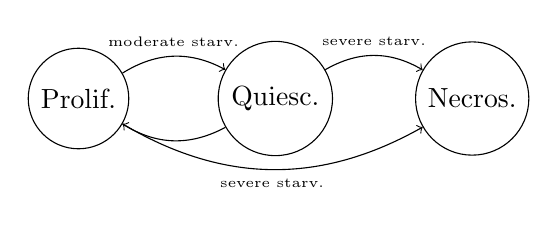
\begin{tikzpicture}
		\node[circle,draw] (P) at (2,0) {Prolif.};
		\node[circle,draw] (Q) at (4.5,0) {Quiesc.};
		\node[circle,draw] (N) at (7,0) {Necros.};
		
		\draw[->] (P) to[bend left] node[above]{\tiny{moderate starv.}} (Q) ;
		\draw[->] (Q) to[bend left] (P); 
		\draw[->] (Q) to[bend left] node[above]{\tiny{severe starv.}} (N); 
		\draw[->] (P) to[bend right] node[below]{\tiny{severe starv.}} (N); 
		\end{tikzpicture}
		
	\column{60mm}
	\only<2->{
	\begin{itemize}
		\item \textbf{Prolif. }: Division + Normal consumption 
		\item \textbf{Quiesc.} : Reduced consumption
		\item \textbf{Necros.} : No consumption
	\end{itemize}
	 }
\end{columns}
\vspace{0.6 cm}

\begin{itemize}
 	\item<3-> Shifts between states triggered by nutrient thresholds
	\item<4-> Discrete levels of consumption and proliferation
\end{itemize}

	\only<5>{\begin{block}{}
		How do all modules interact in a full simulation ?
	\end{block}}
\end{frame}

\begin{frame}
\frametitle{Metabolic Variety : Complete Model}
\begin{center}
	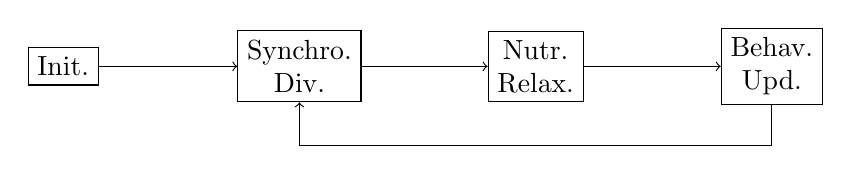
\begin{tikzpicture}
		\node[rectangle,draw,align=center] (I) at (1,0) {Init.};
		\node[rectangle,draw,align=center] (D) at (4,0) {Synchro.\\ Div.};
		\node[rectangle,draw,align=center] (N) at (7,0) {Nutr.\\ Relax.};
		\node[rectangle,draw,align=center] (B) at (10,0) {Behav.\\ Upd.};	
		
		\draw[->] (I)--(D);
		\draw[->] (D)--(N);
		\draw[->] (N)--(B);
		\draw[->] (B) -- (10,-1)  -- (4,-1) -- (D);
	\end{tikzpicture}
\end{center}
\vspace{0.6cm}
\small{
\begin{enumerate}
\item<2-> Performs "division" only to reach a minimal size
\item<3-> "Nutrients" computation until conc. are all stable
\item<4-> Update all cell states according to "Behavior" 
\item<5-> Loops back. Divides all cells in "prolif.". Rearranges agregate 
\item<6-> Repeats "Div.", "Nutr." and "Behav." until the agregate is  large enough
\end{enumerate}
}
\end{frame}

\begin{frame}
\textbf{Now that model structure has been explained, let us use it ! }
\end{frame}
\section{Results}
\subsection{Reference Configuration}

\begin{frame}
\frametitle{Metabolic Variety : Reference configuration}
\underline{Reference Configuration}: 
\begin{itemize}
\item Only growth and nutrients dynamics
\item Useful to choose some parameters 
\item Helpful to understand
\end{itemize}

\end{frame}

\begin{frame}
\frametitle{Metabolic Variety : Reference configuration - Nutrients}
\textbf{Nutrients :  Substrate and Oxygen} 
\vspace{1 cm}
\begin{columns}
\column{60mm}
\underline{Substrate }:
\begin{itemize}
\item Medium Diffusion :  0.3
\item Tissue Diffusion : 0.05
\item Consumption :  ??
\end{itemize}
\column{60mm}
\underline{Oxygen }:
\begin{itemize}
\item Medium Diffusion :  1
\item Tissue Diffusion : 0.6
\item Consumption : ??
\end{itemize}
\end{columns}
\only<2>{\begin{block}{}
	What should be the value for consumption ?
\end{block}}
\end{frame}

\begin{frame}
\frametitle{Metabolic Variety : Reference configuration - Nutrients}
\begin{columns}[T]
\column{30mm}
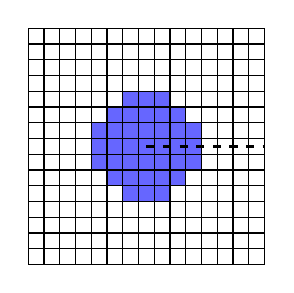
\begin{tikzpicture}
\begin{scope}[scale =2]
	\draw (0,0) grid[step=0.1] (1.5,1.5) rectangle (0,0);
	
    \draw[fill=blue!60!white] (0.5,0.5) grid[step=0.1] (1.0,1.0) rectangle (0.5,0.5);
    \draw[fill=blue!60!white] (0.4,0.6) grid[step=0.1] (1.1,0.9) rectangle (0.4,0.6);
 	\draw[fill=blue!60!white] (0.6,0.4) grid[step=0.1] (0.9,1.1) rectangle (0.6,0.4);
 	\draw[very thick,dashed](0.75,0.75)--(1.5,0.75); 
\end{scope}
\end{tikzpicture}\\

\column{50mm}
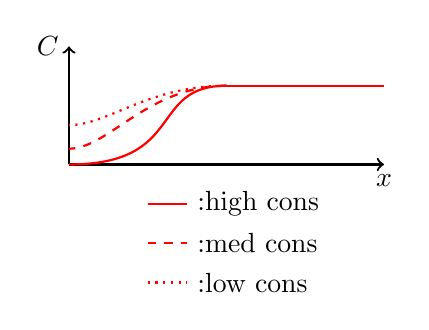
\begin{tikzpicture}
\draw[->,thick] (0,0)--(0,1.5) node[left]{$C$};
\draw[->,thick] (0,0)--(4,0) node[below]{$x$};;
\draw[color=red,thick](2,1) .. controls (1,1) and (1.5,0) .. (0,0);
\draw[color=red,dashed,thick](2,1) .. controls (1,1) and (0.5,0.2) .. (0,0.2);
\draw[color=red,dotted,thick](2,1) .. controls (1,1) and (0.5,0.5) .. (0,0.5);
\draw[color=red,thick](2,1)--(4,1);

\draw[color=red,thick](1,-0.5) -- (1.5,-0.5)node[right,color=black]{:high cons};
\draw[color=red,thick,dashed](1,-1) -- (1.5,-1)node[right,color=black]{:med cons};
\draw[color=red,thick,dotted](1,-1.5) -- (1.5,-1.5)node[right,color=black]{:low cons};
%\draw[domain=4:0,color=red] plot (\x,{\x^4/(1^4+\x^4)});
%\draw[domain=4:0,color=red,dashed] plot (\x,{(\x+1)^4/(2^4+(\x+1)^4)});
\end{tikzpicture}
\end{columns}
\vspace{0.3 cm}
Consumption should be :
\begin{itemize}
\item High enough for a depleted zone to form at $d$ = 1-2 mm
\item Low enough for the transition zone to be large (i.e cover several squares)
\end{itemize}
\end{frame}

\begin{frame}
\frametitle{Metabolic Variety : Reference configuration - Nutrients}
Steady state nutrient concentration for $d= 2$ mm\\
\vspace{0.3cm}

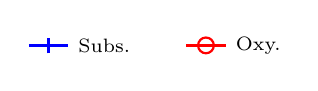
\begin{tikzpicture}
\draw[blue,thick] (0,0)--(1/2,0) node[right,black]{\scriptsize{Subs.}};
\draw[blue,thick] (1/4,-0.1)--(1/4,0.1);
\draw[red,thick] (2,0)--(2+1/2,0)node[right,black]{\scriptsize{Oxy.}};
\draw[red,thick] (2+1/4,0) circle (0.1);
\end{tikzpicture}


\begin{columns}

\column{40mm}
\small
Id:
\input{ref_Id_midl.tex}
\begin{center}
\small
$k_S$ = 0.1\\
$k_O$ =  0.7\\
\end{center}

\column{40mm}
\only<3->{
Ox:
\input{ref_Ox_midl.tex}
\begin{center}
\small
$k_S$ = 0.1\\
$k_O$ =  0.07\\
\end{center}
}
\column{40mm}
\only<4->{
Gl:
\input{ref_Gl_midl.tex}
\begin{center}
\small
$k_S$ = 0.01\\
$k_O$ =  0.7\\
\end{center}
}
\end{columns}
\only<5->{
\begin{block}{}
With these three configurations, most nutrients configurations are adressed
\end{block}
}
\end{frame}

\begin{frame}
\frametitle{Metabolic Variety : Reference configuration - Nutrients}
Now, let us look at the concentration at the center vs time
\vspace{0.3cm}
\begin{columns}[T]
\column{60mm}
\small Substrate :\\
\input{St_ctr_ref_conf.tex}

\column{60mm}
\small Oxygen :\\
\input{Ot_ctr_ref_conf.tex}
\end{columns}
\begin{center}
\begin{tikzpicture}

\draw[thick,cyan!50!blue] (0,0)node[left,black]{\scriptsize Id :}--(1/2,0);
\draw[thick,orange!90!black] (2,0)node[left,black]{\scriptsize Ox :}--(2+1/2,0) ;
\draw[thick,yellow!40!orange] (4,0)node[left,black]{\scriptsize Gl :}--(4+1/2,0) ;
\end{tikzpicture} 
\end{center}
\begin{block}{}
The concentration decreases gradually as the agregate grows
\end{block}
\end{frame}

\subsection{First Study}
%\begin{frame}
%\frametitle{Metabolic Variety : First Study - Growth}
%\begin{columns}
%\column{30mm}

%\begin{tikzpicture}
%\begin{scope}[scale=2]
%	\draw (0,0) grid[step=0.1] (1.5,1.5) rectangle (0,0);
%	
%    \draw[fill=blue!60!white] (0.5,0.5) grid[step=0.1] (1.0,1.0) rectangle (0.5,0.5);
%    \draw[fill=blue!60!white] (0.4,0.6) grid[step=0.1] (1.1,0.9) rectangle (0.4,0.6);
% 	\draw[fill=blue!60!white] (0.6,0.4) grid[step=0.1] (0.9,1.1) rectangle (0.6,0.4);
%\end{scope}	
%\end{tikzpicture}\\
%
%
%\column{60mm}
%\begin{itemize}
%\item  $ \Delta x = 60$ \textmu m
%\item  Starts nutrients dyn. with 16 cells
%\item  Population left to grow until $d_{patch} \approx$ 2 mm 
%\end{itemize}
%\end{columns}
%\end{frame}

%\begin{frame}
%\frametitle{Metabolic Variety : Substrate response}
%
%The first "family" of configurations
%
%\end{frame}
%
%
%\begin{frame}
%\frametitle{Metabolic Variety : Substrate response - Behavior}
%\begin{columns}
% \column{40mm}
% \begin{tikzpicture}
% \begin{scope}[scale=2]	
% 	\draw[fill=green!35!black] (0,0) grid[step=0.1] (1.5,1.5) rectangle (0,0);
%	
%    \draw[fill=green!70!black] (0.5,0.5) grid[step=0.1] (1.0,1.0) rectangle (0.5,0.5);
%    \draw[fill=green!70!black] (0.4,0.6) grid[step=0.1] (1.1,0.9) rectangle (0.4,0.6);
% 	\draw[fill=green!70!black] (0.6,0.4) grid[step=0.1] (0.9,1.1) rectangle (0.6,0.4);
% 		\draw[fill=green!90!black] (0.6,0.6) grid[step=0.1] (0.9,0.9) rectangle (0.6,0.6);
% 		\draw[fill=green!15!white] (0.7,0.7) grid[step=0.1] (0.8,0.8) rectangle (0.7,0.7);
%\end{scope}
%\end{tikzpicture}\\
%
%\vspace{0.3cm}
%B1-B5 are to be specified for each substudy
% 
%\column{60mm}
%\small{
%\begin{itemize}
%\item Substrat : \scriptsize{
%\begin{itemize}
%\item prolif threshold : 50 \% $C_{ext}$
%\item Survival threshold : 20 \% $C_{ext}$
%\end{itemize}
%}
%\item \small{Oxygen :}\scriptsize{
%\begin{itemize}
%\item response threshold : 40 \% $C_{ext}$
%\end{itemize}
%}
%\end{itemize}
%}
%
%\begin{tikzpicture}
%\draw[->,thick] (0,0)--(0,2) node[left]{$[O]$};
%\draw[->,thick] (0,0)--(4,0) node[below]{$[S]$};
%
%\draw[fill=magenta!30!white] (0,0) rectangle node{B5} (0.8,1.8);
%\draw[fill=cyan!30!white] (0.8,0) rectangle node{B4} (0.5*4,0.4*2);
%\draw[fill=green!30!white] (0.5*4,0) rectangle node{B2} (3.8,0.4*2);
%\draw[fill=cyan!30!white] (0.8,0.4*2) rectangle node{B3} (0.5*4,1.8);
%\draw[fill=green!30!white] (0.5*4,0.4*2) rectangle node{B1} (3.8,1.8);
%
%\draw (0.5*4,-0.3) node{$[S]_{prol}$};
%\draw (0.2*4,-0.3) node{$[S]_{surv}$};
%\draw (-0.5,0.5*2) node{$[O]_{resp}$};
%\end{tikzpicture}
%\vspace{0.5 cm}
%\scriptsize{
%\begin{tabular}{|l||l||l|}
%\hline
%    ... & $[S]\geq [S]_{prol}$ & right-aligned \\ 
%\hline
%    $[O]\geq [O]_{resp.}$ & C & E\\ 
%\hline
%    $[O] < [O]_{resp.}$ & D & F\\ 
%\hline
%\end{tabular}
%}

%\end{columns}

%\end{frame}


\begin{frame}
\frametitle{First study : Substrate response}
In order to full understand the model, it is important to start with a simple case and complexify gradually:
\vspace{0.6cm}
\begin{enumerate}
	\item<2-> No response 
		\only<3>{
		\begin{itemize}
		\item Cells consume w/o responding to nutrients
		\end{itemize}
		}
	\item<4-> Starvation
		\only<5>{
		\begin{itemize}
		\item Cells can starve and die
		\end{itemize}
		}
	\item<6-> Savy 
		\only<7>{
		\begin{itemize}
		\item Cells can starve and die
		\item They start consuming less nutrient 
		\item They stop proliferation in moderate starvation
		\end{itemize}
		}
	\item<8-> Compensation
		\only<9>{
		\begin{itemize}
		\item Cells can starve and die
		\item They start consuming less substrate
		\item They stop proliferation in moderate starvation
		\item Cell start consuming more oxygen to make up for loss energy 
		\end{itemize}
		}
	\item<10-> Compensation + Proliferation
		\only<11>{
		\begin{itemize}
		\item Cells can starve and die
		\item They start consuming less substrate
		\item They stop proliferation in moderate starvation
		\item Cell start consuming more oxygen to make up for loss energy 
		\item Cell
		\end{itemize}
		}
\end{enumerate}
\only<12>{\begin{block}{}
		Now, let us look at population and nutrients dynamics in those cases.
	\end{block}}
\end{frame}


\begin{frame}
\frametitle{ Substrate response : Population dynamics}
\begin{center}
\begin{columns}
\column{50mm}
\input{Ox_lives.tex}
\column{50mm}
\input{Ox_deads.tex}
\end{columns}
\end{center}
\begin{itemize}
\item Quiescence $\rightarrow$ "irregular" growth \& less cell death
\item Faster growth w/o quiescence
\end{itemize} 
\end{frame}

%\begin{frame}
%\frametitle{ Substrate response : Population dynamics}
%\begin{center}
%\begin{columns}
%\column{50mm}
%\input{Gl_lives.tex}
%\column{50mm}
%\input{Gl_deads.tex}
%\end{columns}
%\end{center}
%\begin{itemize}
%\item Quiescence -> "irregular" growth \& less cell death
%\item Faster growth w/o quiescence
%\end{itemize} 
%\end{frame}

\begin{frame} 
\frametitle{ Substrate response : Nutrient dynamics}
\begin{center}
\begin{columns}
\column{50mm}
\input{St_ctr_Ox.tex}
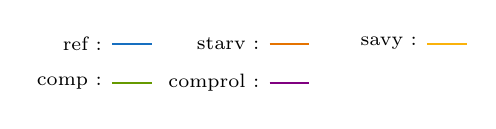
\begin{tikzpicture}
\draw[thick,cyan!50!blue] (0,0)node[left,black]{\scriptsize ref :}--(1/2,0);
\draw[thick,orange!90!black] (2,0)node[left,black]{\scriptsize starv :}--(2+1/2,0) ;
\draw[thick,yellow!40!orange] (4,0)node[left,black]{\scriptsize savy :}--(4+1/2,0) ;
\draw[thick,red!40!green] (0,-1/2)node[left,black]{\scriptsize comp :}--(0+1/2,-1/2) ;
\draw[thick,red!50!blue] (2,-1/2)node[left,black]{\scriptsize comprol :}--(2+1/2,-1/2) ;
\end{tikzpicture} 
\end{columns}
\end{center}
\end{frame}

\end{document}
